\chapter{Literature overview}\label{ch:literature-overview}

In \cite{kandasamyEffectiveLocationMicro2020} authors proposed solution to cutting problem.
They describe it as cutting multiple parts from metal sheet using cutting tool.
The main focus is on preventing cutted parts from falling out of the metal sheet.
They use micro-joints to solve this problem. Micro-joint is part of the cutting tool
path that is not cutted – holding part and preventing it from falling.

This presents multitude of problems that they address by using genetic algorithm
and heuristic. Chromosome is genetic string with two parts – first holds
angle values and second holds segment numbers. Using this representation they are able
to map (using simple heuristic) each individual to one cutting tool path and micro-joint positions.
Fitness and objective are minimize air travel distance for the cutting tool needed to cut the
path. They used standard operators – two point partial matching crossover and mutation
as swapping chromosome genes.

According to the authors they achieved "near optimal" results in comparison with randomly
generated solutions and industry standards for cutting sheet metal parts.

In \cite{vijayanandHeuristicGeneticApproach2015} authors solved similar problem. They it
as placing squares to the grid with two optimization criterions – minimize air travel distance
for the cutting tool needed to cut the path (same as above), minimize unused are of the grid (different from above).
Formulation of this problem is closely related to 2SLOPP\footnotemark

WIP: Summary of "Review of the cutting path algorithms" \cite{dewilReviewCuttingPath2016}.


\begin{figure}[htp]
    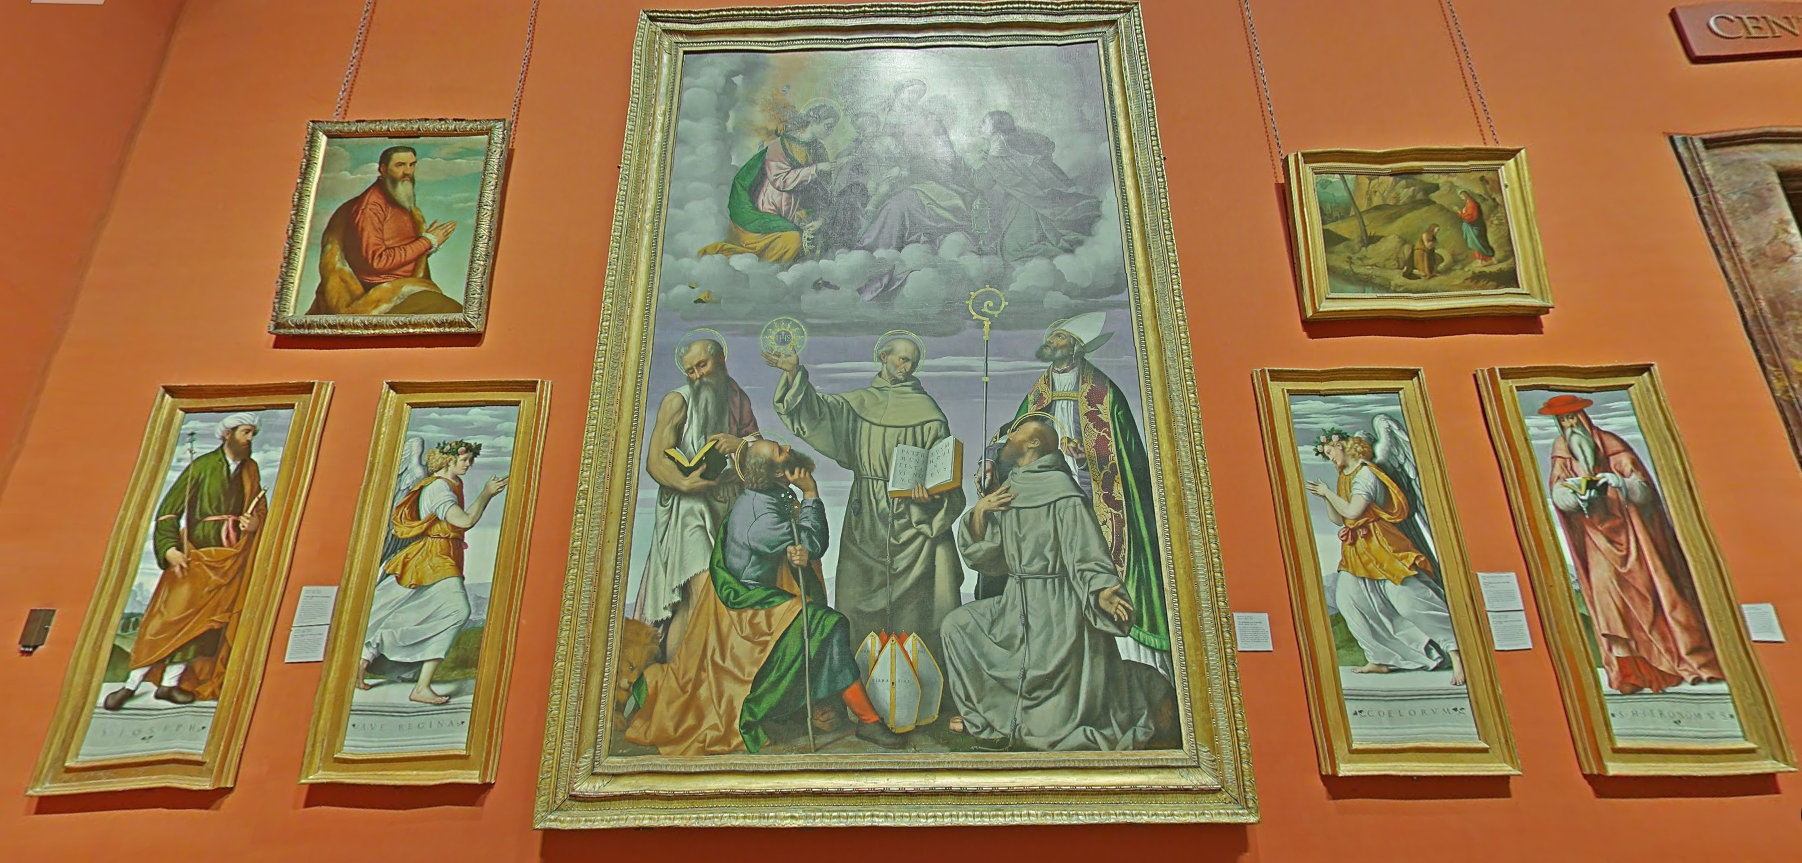
\includegraphics[width=1\textwidth, left]{london_gallery_wall}
    \caption{Painting placement at the The National Gallery, London. Source:~\cite{ScreenshotWallGoogle}}
    \label{fig:london-wall}
\end{figure}

\footnotetext{Two dimensional single large object placement problem}

